  % $Id: TimeMgr_desc.tex,v 1.26 2009/02/13 15:45:48 murphysj Exp $

The ESMF Time Manager utility includes software for time and date 
representation and calculations, model time advancement, and the 
identification of unique and periodic events.  Since multi-component 
geophysical applications often require synchronization across
the time management schemes of the individual components, the 
Time Manager's standard calendars and consistent time representation 
promote component interoperability.
\begin{center}  
\begin{tabular}{|p{6in}|}
\hline
\vspace{.01in}
{\bf Key Features} \\[.01in]
Drift-free timekeeping through an integer-based internal time 
representation.  Both integers and reals can be specified at the interface. \\
The ability to represent time as a rational fraction, to support 
exact timekeeping in applications that involve grid refinement. \\
Support for many calendar types, including user-customized calendars. \\
Support for both concurrent and sequential modes of component execution. \\
Support for varying and negative time steps. \\[.03in] \hline
\end{tabular}
\end{center}

\subsection{Time Manager Classes}
There are five ESMF classes that represent time concepts:
\begin{itemize}
\item {\bf Calendar}  A Calendar can be used to keep track of the 
date as an ESMF Gridded Component advances in time. Standard calendars 
(such as Gregorian and 360-day) and user-specified calendars are 
supported.  Calendars can be queried for quantities such as seconds 
per day, days per month, and days per year.  
\item {\bf Time} A Time represents a time instant in a particular
calendar, such as November 28, 1964, at 7:31pm EST in the Gregorian 
calendar.  The Time class can be used 
to represent the start and stop time of a time integration.
\item {\bf TimeInterval} TimeIntervals represent a period 
of time, such as 300 milliseconds.  Time steps can be represented 
using TimeIntervals.  
\item {\bf Clock} Clocks collect the parameters and 
methods used for model time advancement into a convenient 
package.  A Clock can be queried for quantities such
as start time, stop time, current time, and time step.  Clock
methods include incrementing the current time, and determining
if it is time to stop.  
\item {\bf Alarm} Alarms identify unique or periodic events
by ``ringing'' - returning a true value - at specified times.  
For example, an Alarm might be set to ring on the day of the 
year when leaves start falling from the trees in a climate model.
\end{itemize}

\begin{center}
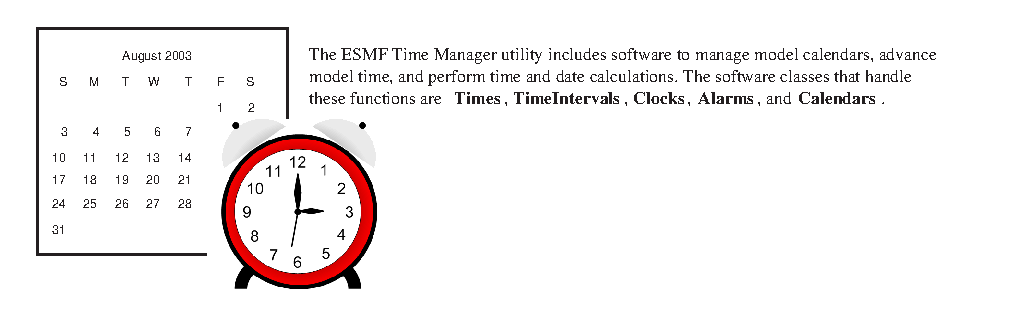
\includegraphics{TimeMgr_desc}
\end{center}

\newpage
In the remainder of this section, we briefly summarize the 
functionality that the Time Manager classes provide.  Detailed 
descriptions and usage examples precede the API listing for each 
class.

\subsection{Calendar}
An ESMF Calendar can be queried for seconds per day, days per month 
and days per year.  The flexible definition of Calendars allows them
to be defined for planetary bodies other than Earth.  The set of supported 
calendars includes:
\begin{description}
\item [Gregorian] The standard Gregorian calendar.
\item [no-leap] The Gregorian calendar with no leap years.
\item [Julian] The standard Julian date calendar.
\item [Julian Day] The standard Julian days calendar.
\item [Modified Julian Day] The Modified Julian days calendar.
\item [360-day] A 30-day-per-month, 12-month-per-year calendar.
\item [no calendar] Tracks only elapsed model time in hours, minutes, seconds.
\end{description}
See Section~\ref{sec:Calendar} for more details on supported standard 
calendars, and how to create a customized ESMF Calendar.

\subsection{Time Instants and TimeIntervals}

\label{subsec:Time Instants and TimeIntervals}
TimeIntervals and Time instants (simply called Times) are the computational 
building blocks of the Time Manager utility.  TimeIntervals support operations
such as add, subtract, compare size, reset value, copy value, and subdivide
by a scalar.  Times, which are moments in time associated with specific
Calendars, can be incremented or decremented by TimeIntervals, compared to
determine which of two Times is later, differenced to obtain the TimeInterval
between two Times, copied, reset, and manipulated in other useful ways.
Times support a host of different queries, both for values of individual Time 
components such as year, month, day, and second, and for derived values such 
as day of year, middle of current month and Julian day.  It is also possible 
to retrieve the value of the hardware realtime clock in the form of a 
Time.  See Sections~\ref{sec:Time} and ~\ref{sec:TimeInterval}, respectively,
for use and examples of Times and TimeIntervals.

Since climate modeling, numerical weather prediction and other 
Earth and space applications have widely varying time scales and require 
different sorts of calendars, Times and TimeIntervals must support 
a wide range of time specifiers, spanning nanoseconds to years.  The
interfaces to these time classes are defined so that the user can specify a time
using a combination of units selected from the list shown in 
Table~\ref{table:timeOpts}.  

\subsection{Clocks and Alarms}
Although it is possible to repeatedly step a Time forward by a 
TimeInterval using arithmetic on these basic types, it is useful to 
identify a higher-level concept to represent this function.  We refer to 
this capability as a Clock, and include in its required features the 
ability to store the start and stop times of 
a model run, to check when time advancement should cease, 
and to query the value of quantities such as the current time and the
time at the previous time step.  The Time Manager includes a class 
with methods that return a true value when a periodic or unique event 
has taken place; we refer to these as Alarms.  Applications may contain 
temporary or multiple Clocks and Alarms.  Sections~\ref{sec:Clock} and
\ref{sec:Alarm} describe the use of Clocks and Alarms in detail.






